\pgfsetplotmarksize{0pt}
\begin{figure}
 \centering
 \caption{\label{fl_conv4}FLClustered/test4.txt},
 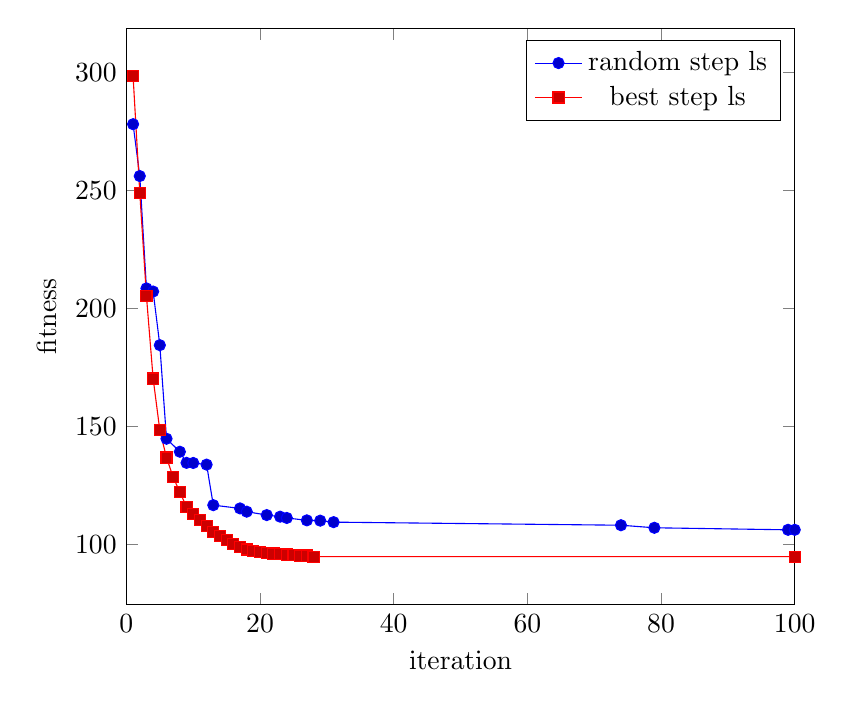
\begin{tikzpicture}
 \begin{axis}[
   width=0.7\textwidth,
   scale only axis,
   xlabel=iteration,
   ylabel=fitness,
   xmin=0,xmax=100,
   domain=0:100]
   \addplot coordinates {
     (0,inf)
     (1,277.93)
     (2,255.961)
     (3,208.387)
     (4,207.051)
     (5,184.342)
     (6,144.707)
     (8,139.194)
     (9,134.491)
     (10,134.449)
     (12,133.736)
     (13,116.575)
     (17,115.194)
     (18,113.819)
     (21,112.371)
     (23,111.699)
     (24,111.153)
     (27,110.136)
     (29,110.006)
     (31,109.378)
     (74,108.072)
     (79,106.989)
     (99,106.128)
     (100,106.128)
   };
   \addlegendentry{random step ls}
   \addplot coordinates {
     (0,inf)
     (1,298.231)
     (2,248.912)
     (3,205.082)
     (4,170.206)
     (5,148.277)
     (6,136.741)
     (7,128.409)
     (8,122.085)
     (9,115.833)
     (10,112.719)
     (11,110.175)
     (12,107.708)
     (13,105.32)
     (14,103.469)
     (15,101.789)
     (16,100.258)
     (17,98.7572)
     (18,97.7929)
     (19,97.135)
     (20,96.7303)
     (21,96.383)
     (22,96.0772)
     (23,95.9544)
     (24,95.6631)
     (25,95.3391)
     (26,95.2303)
     (27,95.2262)
     (28,94.7727)
     (100,94.7727)
   };
   \addlegendentry{best step ls}
 \end{axis}
 \end{tikzpicture}
\end{figure}
